\documentclass{article}

% Essential packages
\usepackage{graphicx}   % For image handling
\usepackage{subcaption} % For multi images
\usepackage{caption}    % For proper captions
\usepackage{listings}   % For code listings
\usepackage{fontspec}   % For custom fonts
\usepackage{xcolor}     % For color support
\usepackage{tcolorbox}  % For code block boxes
\usepackage{etoolbox}   % For patching and command manipulation
\usepackage{titlesec}   % For section formatting
\usepackage{parskip}    % For customisable paragraph formating
\usepackage{comment}    % For being able to comment out sections
\usepackage{geometry}   % For managing page size and margins
\usepackage{hyperref}   % For embedding links, like URL's
\usepackage{bigstrut}
\usepackage{multirow}
\usepackage{colortbl}
\usepackage{amsmath}    % For math and equation formatting

\tcbuselibrary{listings, skins, breakable}  %Librarary to make code blocks multipage


%   ############################## Customisation ##############################

% Document metadata
\title{\fontsize{24}{36}\selectfont Programable Logic Circuts\\ %Edit title here \\ means new line
Lab 04} % Line 2 of title, its not subtitle, that is possible to, google it
\author{{\ttfamily Sølve Kjelseth}} % Input your name, replace \ttfamily with \normalfont to make it not monospaced but regular font (removing \ttfamily will not do this because of the monospaced font inside tables command, and author is technically a 1x1 table)
\date{\today} % Auto updates the date, untill you export it, replace with hardcoded date if you need

% Adjust the body text font size to 12pt without affecting section headings
\renewcommand{\normalsize}{\fontsize{12}{16}\selectfont}

% Adjust the paragraph spacing, either as indentation or/and line spaceing
\setlength{\parindent}{0pt}  % Remove indentation
\setlength{\parskip}{6pt}    % Add vertical space between paragraphs

% Customisation of fonts and colors
\setmainfont{Times New Roman}
\setmonofont{JetBrains Mono}
\definecolor{background}{RGB}{225, 219, 202}
\definecolor{darkAccent}{RGB}{140, 98, 64}
\definecolor{commentGreen}{RGB}{26, 159, 32}
\definecolor{keywordPurple}{RGB}{229, 24, 192}
\definecolor{keywordBlue}{RGB}{5, 142, 217}
\definecolor{portOrange}{RGB}{234, 72, 31}
\definecolor{darkGray}{RGB}{60, 60, 60}

% Link color customization
\hypersetup{
    colorlinks=true,
    linkcolor=darkGray, % Internal links such as table of contents or figure referencing
    urlcolor=keywordBlue % URL colors
    }
\urlstyle{same} % Makes url in the same style as the rest of the document

% Customisation of margins and paper size
\geometry{
 a4paper,
 left = 30mm,
 right = 30mm,
 top = 30mm,
 bottom = 30mm
 }

% Sections formatting and numbering
% Sets the font to monospace for section, subsection and subsubsection
% and sets the format to be numbers with . between and at the end
\renewcommand{\thesection}{\texttt{\arabic{section}.}}
\renewcommand{\thesubsection}{\texttt{\arabic{section}.\arabic{subsection}.}}
\renewcommand{\thesubsubsection}{\texttt{\arabic{section}.\arabic{subsection}.\arabic{subsubsection}.}}

\setcounter{section}{-1}  % Start section numbering from 0, delete this to start from 1


\newcounter{codeblock} % Define new counter
\renewcommand{\thecodeblock}{\arabic{section}.\arabic{codeblock}} % Define numbering format

% Makes section monospace font and start each subsection from 0 and figure number
\let\oldsection\section
\renewcommand{\section}[1]{%
  \oldsection{\texttt{#1}} % Make section title monospace
  \setcounter{subsection}{-1} % Makes subsection start from 0, delete this line to start from 1
  \setcounter{figure}{-1} % Makes figure numbers start from 0, delete this line to start from 1
  \setcounter{table}{-1} % Makes table numbers start from 0, delete this line to start from 1
  \setcounter{codeblock}{-1}
}


% Makes subsection monospace font and start each subsubsection from 0
\let\oldsubsection\subsection
\renewcommand{\subsection}[1]{%
  \oldsubsection{\texttt{#1}}% Make subsection title monospace
  \setcounter{subsubsection}{-1}% Makes subsubsection start from 0, delete this line to start from 1
}

% Makes subsubsection monospace font
\let\oldsubsubsection\subsubsection
\renewcommand{\subsubsection}[1]{%
  \oldsubsubsection{\texttt{#1}}% Make subsubsection title monospace
}

% Makes every new section start on a new page, except for the first section, section 0
\pretocmd{\section}{%
  \ifnum\value{section}=-1 \else\clearpage\fi % Replace -1 with 0 if sections start at nr. 1
}{}{}

% Makes Table of contents a subsection
\makeatletter
\renewcommand{\tableofcontents}{%
    \subsection{Table of Contents} % Numbered subsection named Table of contents
    \@starttoc{toc}%
}
\makeatother

% Makes List of figures a subsection
\makeatletter
\renewcommand{\listoffigures}{%
    \subsection{List of Figures} % Numbered subsection named List of figures
    \@starttoc{lof}%
}
\makeatother

% Makes List of tables a subsection
\makeatletter
\renewcommand{\listoftables}{%
    \subsection{List of Tables} % Numbered subsection named List of tables
    \@starttoc{lot}%
}
\makeatother


% Makes every figure be formated as section number.figure number
\renewcommand{\thefigure}{\arabic{section}.\arabic{figure}}

% Makes every table be formated as section number.table number
\renewcommand{\thetable}{\arabic{section}.\arabic{table}}
\AtBeginEnvironment{tabular}{\ttfamily} % Monozpaced font within tables

% Add keywords to be highlited in blue below. Note that all reserved
% keywords from VHDL is already in purple and should not be added here
% too as duplicates will cause issues. Therfore compile this document
% after pasting in code and only add non-highlited words to this list.
% Also, there is not a list for orange keywords, used for ports here.
\lstdefinelanguage{VHDL+}{
    language     = VHDL,
    morestring = [b]',
    morekeywords = [2]{
        IEEE,
        std_logic_1164, std_logic, std_logic_vector},
    morekeywords = [3]{
        SW, LEDR, KEY,
        HEX0, HEX1, HEX2, HEX3, HEX4, HEX5, HEX6},
    sensitive = false
}


%   ############################## Advanced customisation ##############################

% Customisation of list style inside code block
\lstdefinestyle{VHDL}{
    language = VHDL+, % Uses the extra higlights from above
    % The folloowing lines defines color for highlighting, other changes like
    % italic, bold or different fonts can also be added to this
    escapechar = §,
    commentstyle = \color{commentGreen}, 
    keywordstyle = \color{keywordPurple},
    keywordstyle = [2]\color{keywordBlue},
    keywordstyle = [3]\color{portOrange},
    stringstyle = \color{darkAccent},
    basicstyle = \ttfamily\small, % Default font inside code block
    numberstyle = \ttfamily\color{darkAccent}, % Style of line numbering
    numbers = left, % Line numbering on left side
    breakatwhitespace = false, % Don't start new line with only whitspaces
    breaklines = true, % If line is to long it will wrap to next line (line number does not increase)
    keepspaces = true, % Indents works logical
    showspaces = false, % Space is blank character, set to true to show dots instad
    showstringspaces = false, % Same as above but inside strings
    showtabs = false, % Tab is also blank character, set to true to show dashes
    tabsize = 4, % Tabsize is set to 4, this works well with code from notepad++
    % Dont mess with the ones below unless you want to mess with the box as well
    % These took some time to line up such that it looks natural
    numbersep = 10pt, % Adjust distance between numbers and code
    xleftmargin = -8pt,% Negative margin to pull code text closer to the left border
}

% This is for code where VHDL is not an argument
\lstdefinestyle{Example Code}{
    basicstyle = \ttfamily\small, % Default font inside code block
    numberstyle = \ttfamily\color{darkAccent}, % Style of line numbering
    numbers = left, % Line numbering on left side
    breakatwhitespace = false, % Don't start new line with only whitspaces
    breaklines = true, % If line is to long it will wrap to next line (line number does not increase)
    keepspaces = true, % Indents works logical
    showspaces = false, % Space is blank character, set to true to show dots instad
    showstringspaces = false, % Same as above but inside strings
    showtabs = false, % Tab is also blank character, set to true to show dashes
    tabsize = 4, % Tabsize is set to 4, this works well with code from notepad++
    % Dont mess with the ones below unless you want to mess with the box as well
    % These took some time to line up such that it looks natural
    numbersep = 10pt, % Adjust distance between numbers and code
    xleftmargin = -8pt,% Negative margin to pull code text closer to the left border
}

\lstset{style = Example Code} %Sets the default style to Example Code

% Customisation of code block itself
\newtcolorbox[auto counter, number within=section]{codeBlock}[2][]{
    colback=background, % Background color for the code block
    colframe=darkAccent, % Border color for the code block
    listing only, %Makes it contain the listing
    arc=10pt, % Rounded corners size
    sharp corners=northeast, % Make top-right corner sharp for the main box
    enhanced jigsaw, % Essential dont mess with it
    breakable, % Allows content to be multipage
    top=-4pt, % Made to line up text dont mess with it
    bottom=-4pt, % Same as above
    before skip=0pt, after skip=10pt, % Adjust spacing before and after the box
    boxrule=1pt, % Border thickness of the main box
    overlay unbroken and first={\node[ % Create label box in the top-right corner
        anchor=north east,      %Position of box, same as sharp corner in this case
        fill=background,        %Background color same as main box
        draw=darkAccent,        %Outline color, same as main box
        line width=1pt,         %Outline thickness, same as main box
        text=keywordPurple,     %Text color
        font=\ttfamily,         %Text font and size
        inner sep=6pt,          %Spacing inside
        minimum width=16pt,     %Minimum box with, it autoresizes depending on text
        minimum height=12pt,    %Minimum box height, it autoresizes depending on text
        text centered,          %Centres the text with the spacing
        sharp corners]          %Makes corners sharp
        at ([xshift=0pt, yshift=0pt]frame.north east) % Position, aligned with corner on main box
        {#2}; % Types your argument in the top corner as a label
    }
}

\newcommand{\writecode}[3][Example Code]{%
    \par\medskip % Adds some vertical spacing before the caption
    \refstepcounter{codeblock} % Step the figure counter
    \label{Code:#2} % Unique label for referencing
    \begin{center} % Center the caption
        Code \thecodeblock: #3 % Fake caption
    \end{center}
    \addcontentsline{lof}{figure}{Code \thecodeblock: #3} % Manually add entry to List of Figures
    \par\medskip % Adds some vertical spacing after the caption before the code block
    \begin{codeBlock}{#1}% arg 1 (default Example Code) will be written in the top right corner box
        \lstinputlisting[style=#1]{Code/#2}% arg 1 style is used and arg 2 is filename
    \end{codeBlock}%
    \par\medskip % Adds some vertical spacing after the code block
}




\newcommand{\figcaption}[1]{%
    \caption[]{#1} % Suppress the default entry in LoF
    \addcontentsline{lof}{figure}{Figure \thefigure: #1} % Manually add the correct format
}

\newcommand{\tabcaption}[1]{%
    \caption[]{#1} % Suppress the default entry in LoT
    \addcontentsline{lot}{table}{Table \thetable: #1} % Manually add the correct format
}

\newcommand{\unit}[1]{\ensuremath{\, \mathrm{#1}}}

\newcommand{\linkgithub}[1]{\href{https://github.com/Kjelseth/PLK_lab.git}{#1}}



%   ############################## Document begins here ##############################
\begin{document}

\maketitle % Makes title front page based on the title, author and date metadata, change at the top



%   ############################## Section ##############################
\addtocontents{toc}{\protect\setcounter{tocdepth}{0}} % Temporarily hide from TOC
\section{Introduction} % Numbered section named Introduction
This is the fourth report in this course, detailing the completion of the fourth lab exercise. With the purpose is to investigate counters.\par
Note: As always, the VHDL and \LaTeX\ code is open source, see
\linkgithub{my GitHub {
\begingroup
\setbox0=\hbox{\includegraphics[scale=0.5]{Figures/github-mark.png}}%
\parbox{\wd0}{\box0}
\endgroup}}
\clearpage
\tableofcontents % Generate TOC
%\clearpage
\listoffigures % List of figures
%\listoftables % List of tables
\addtocontents{toc}{\protect\setcounter{tocdepth}{2}} % Restore TOC depth



%   ############################## Section ##############################
\section{Part 1}
This Part is about making a structural coded counter using T-flip-flop instances and displaying the counted value on some 7-segment displays.


\subsection{Solving}
Solving this task was done by first making a T-flip-flop, as the task did not specify how this should be made, the choice of behavioural code was made. Then the counter was made as described in the task with structural code using eight instances of the T-flip-flop. The display component, code~\ref{Code:Part1_Display.vhd} and its decoder component, code~\ref{Code:Decoder.vhd} was copied from previous lab tasks. Then finally a TLE was made that simply connected the switches and button to the counter and connected the counter to the display.


\clearpage
\subsection{Code}

\writecode[VHDL]{Part1_TLE.vhd}{TLE for the structural counter}

\clearpage
\writecode[VHDL]{Part1_Counter.vhd}{Counter component used in the TLE}

\clearpage
\writecode[VHDL]{Part1_Tff.vhd}{T-flip-flop component used in counter}
\writecode[VHDL]{Part1_Display.vhd}{Display component used in the TLE}

\clearpage
\writecode[VHDL]{Decoder.vhd}{Decoder component used in the display}


\clearpage
\subsection{RTL}
The expanded RTL of the decoder components is not included as it is not relevant for the purpose of this Lab. Check out the \linkgithub{GitHub} at {\small\verb|PLK_lab/Lab03/Temp/Part5_RTL_Display.pdf|} for the RTL, and for more  general information regarding this component, check out\\ {\small\verb|PLK_lab/Lab03/main.tex|} and read part 5 in the rendered document.

\begin{figure}[h]
    \centering
    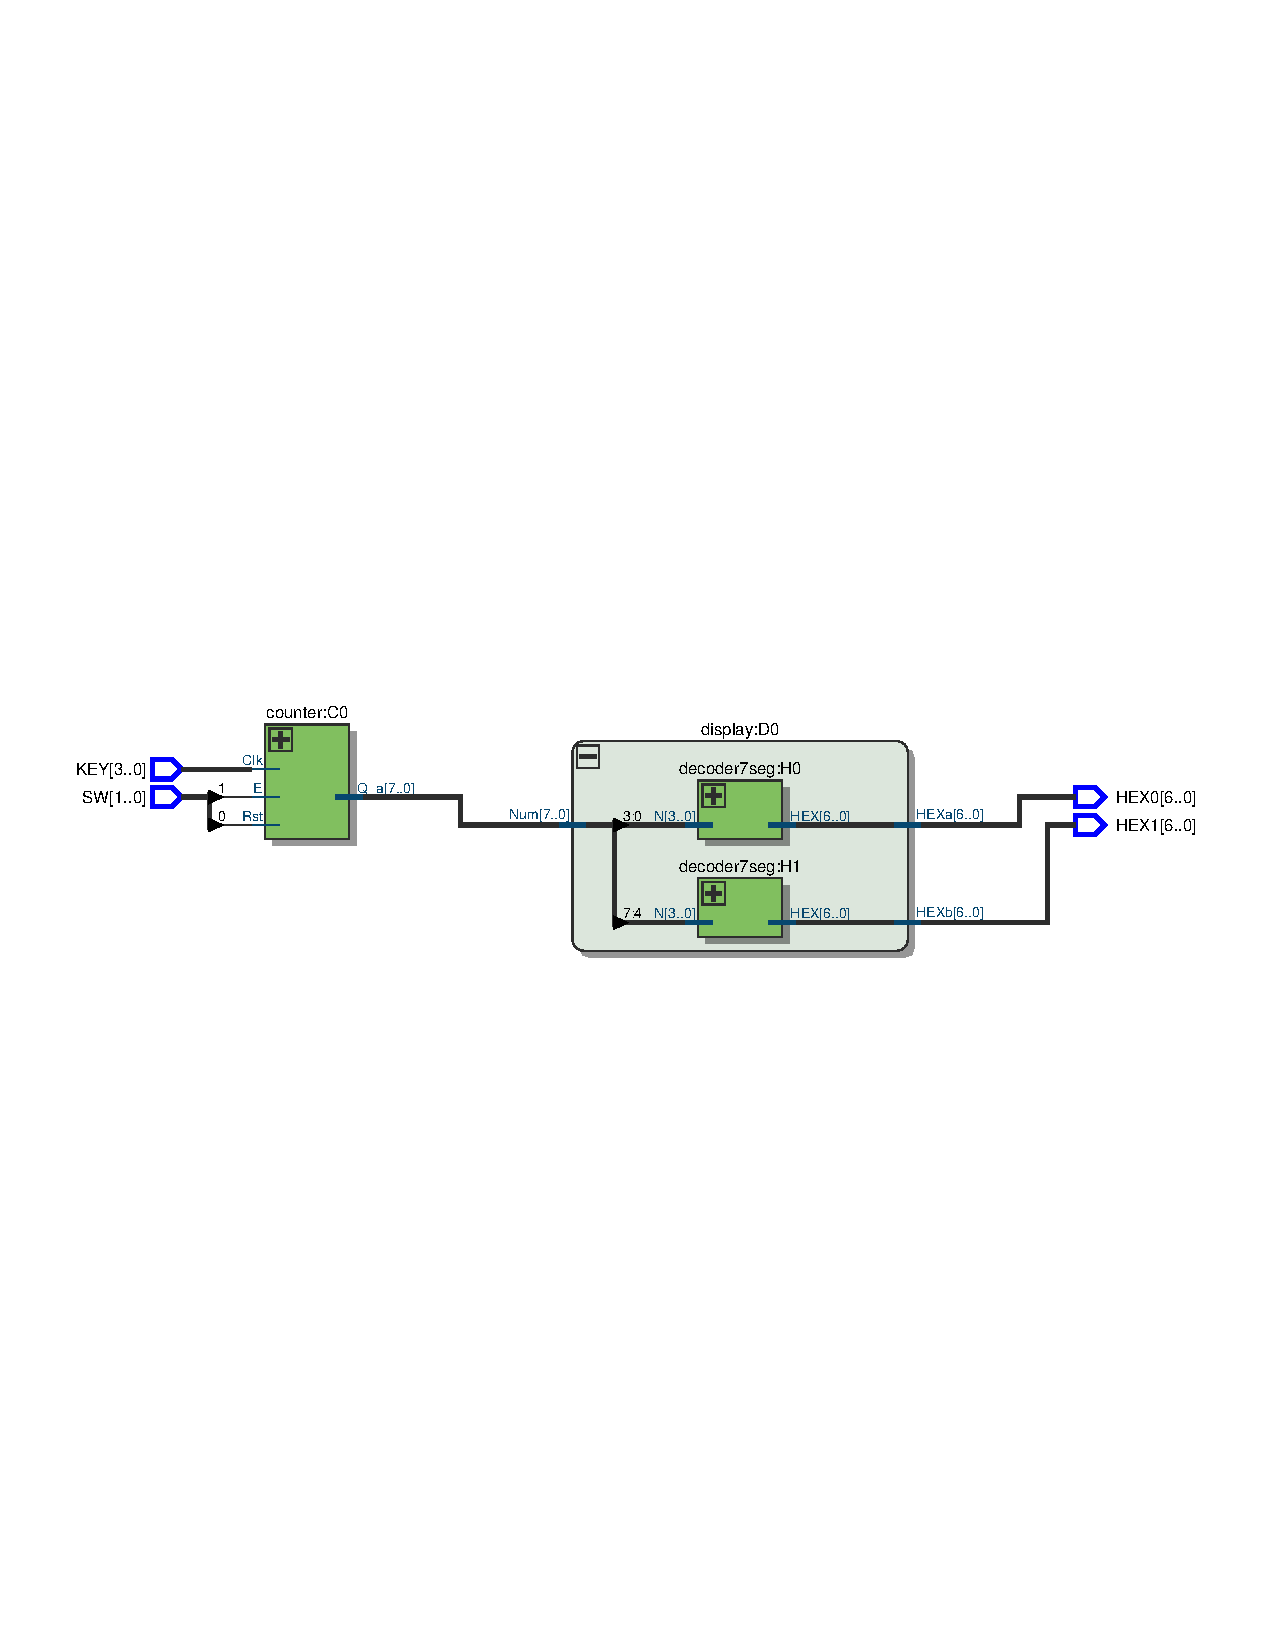
\includegraphics[width=1\textwidth]{Figures/Part1_RTL_TLE.jpg}
    \figcaption{RTL of the TLE}
    \label{fig:p1_RTL_TLE}
\end{figure}

\begin{figure}[h]
    \centering
    \includegraphics[width=1\textwidth]{Figures/Part1_RTL_counter.jpg}
    \figcaption{RTL for the counter used in the TLE}
    \label{fig:p1_RTL_counter}
\end{figure}

\clearpage
\begin{figure}[h]
    \centering
    \includegraphics[width=1\textwidth]{Figures/Part1_RTL_Tff.jpg}
    \figcaption{RTL for the T-flip-flop used in the counter}
    \label{fig:p1_RTL_Tff}
\end{figure}


\clearpage
\subsection{Results}
As read from figure~\ref{fig:p1_comp}, under "Logic utilization", this circuit uses a total of 13 logic elements to realize this configuration.

\begin{figure}[h]
    \centering
    \includegraphics[width=1\textwidth]{Figures/Part1_compiled.jpg}
    \figcaption{Compilation results from structural counter}
    \label{fig:p1_comp}
\end{figure}

\clearpage
\begin{figure}[h]
    \centering
    \begin{subfigure}[t]{0.45\textwidth}
        \centering
        \includegraphics[width=0.8\textwidth]{Figures/Part1_1.jpg}
        \caption{Disabled, reset low, no change}
        \label{fig:p1_1}
    \end{subfigure}
    \hfill
    \begin{subfigure}[t]{0.45\textwidth}
        \centering
        \includegraphics[width=0.8\textwidth]{Figures/Part1_2.jpg}
        \caption{Enabled, reset high, no change}
        \label{fig:p1_2}
    \end{subfigure}

    \begin{subfigure}[t]{0.45\textwidth}
        \centering
        \includegraphics[width=0.8\textwidth]{Figures/Part1_3.jpg}
        \caption{Clock cycle 1, counts up}
        \label{fig:p1_3}
    \end{subfigure}
    \hfill
    \begin{subfigure}[t]{0.45\textwidth}
        \centering
        \includegraphics[width=0.8\textwidth]{Figures/Part1_4.jpg}
        \caption{Clock cycle 2, counts up}
        \label{fig:p1_4}
    \end{subfigure}

    \begin{subfigure}[t]{0.45\textwidth}
        \centering
        \includegraphics[width=0.8\textwidth]{Figures/Part1_5.jpg}
        \caption{Reset low, no change}
        \label{fig:p1_5}
    \end{subfigure}
    \hfill
    \begin{subfigure}[t]{0.45\textwidth}
        \centering
        \includegraphics[width=0.8\textwidth]{Figures/Part1_6.jpg}
        \caption{Clock cycle 3, resets to 0}
        \label{fig:p1_6}
    \end{subfigure}

    \begin{subfigure}[t]{0.45\textwidth}
        \centering
        \includegraphics[width=0.8\textwidth]{Figures/Part1_7.jpg}
        \caption{Enabled, clock cycle \(n\), counts up}
        \label{fig:p1_7}
    \end{subfigure}
    \hfill
    \begin{subfigure}[t]{0.45\textwidth}
        \centering
        \includegraphics[width=0.8\textwidth]{Figures/Part1_8.jpg}
        \caption{Disabled, clock cycle \(n\!+\!1\), no change}
        \label{fig:p1_8}
    \end{subfigure}

    \figcaption{Some functional tests, works as expected}
    \label{fig:p1_results}
\end{figure}



%   ############################## Section ##############################
\section{Part 2}
This is part is about making a similar circuit as part 1 but instead making it with a behavioural code and in 16-bit.


\subsection{Solving}
The behavioural code to make a simple resettable counter was so small that it was made inside the TLE. The statement supplied in the task combined with a simple if statement was enough to make the counter, then a similar pair for clearing the value was also made. instead of splitting the 16-bit number in two, the display component was slightly modified to accept a 16 bit number and use four instances of the decoder instead.


\clearpage
\subsection{Code}

\writecode[VHDL]{Part2_TLE.vhd}{TLE for the behavioural counter}

\clearpage
\writecode[VHDL]{Part2_Display.vhd}{Modified display component used in the TLE}

\clearpage
\subsection{RTL}
Figure~\ref{fig:p2_RTL_TLE} shows that this is implemented using two sets of comparators in series, the first for checking the enable and then count up using an adder each clock cycle. The second for checking the reset and replace the whole number with 0 if reset is low.

\begin{figure}[h]
    \centering
    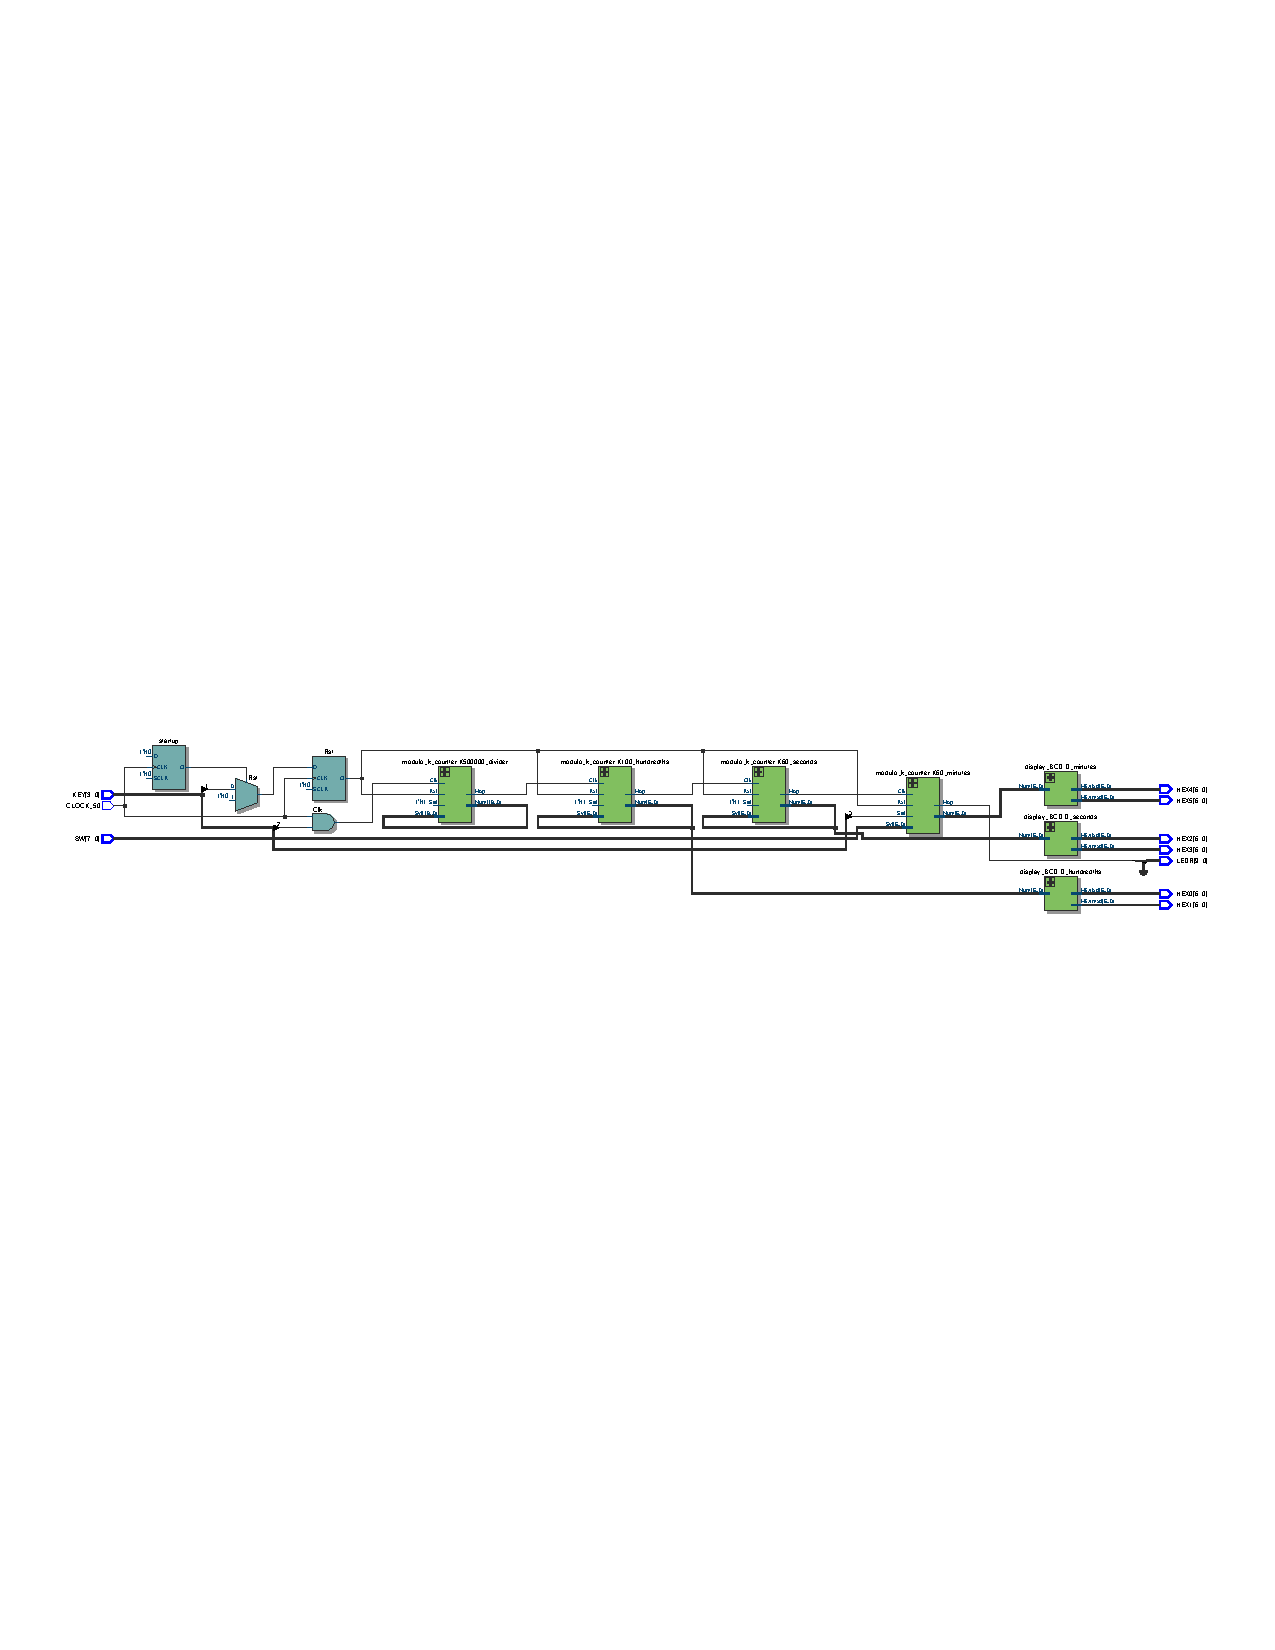
\includegraphics[width=1\textwidth]{Figures/Part2_RTL_TLE.jpg}
    \figcaption{RTL of the TLE}
    \label{fig:p2_RTL_TLE}
\end{figure}


\clearpage
\subsection{Results}
As read from figure~\ref{fig:p2_comp}, under "Logic utilization", this circuit uses a total of 23 logic elements to realize this configuration. Not much different from the structural code in part 1, especially since this is 16-bit and not 8-bit and twice the amount of 7-segment displays. An argument of this being more efficient/compact could be made, but there would be a better comparison if equal circuits were compared.

\begin{figure}[h]
    \centering
    \includegraphics[width=1\textwidth]{Figures/Part2_compiled.jpg}
    \figcaption{Compilation results from behavioural counter}
    \label{fig:p2_comp}
\end{figure}

The pictures from the testing in figure~\ref{fig:p2_results} of this circuit are unfortunately very limited, but it was tested thoroughly off camera to ensure that it worked the way as the part 1 circuit, with the only change being compatibility for larger numbers. 

\clearpage
\begin{figure}[h]
    \centering
    \begin{subfigure}[t]{1\textwidth}
        \centering
        \includegraphics[width=0.65\textwidth]{Figures/Part2_1.jpg}
        \caption{Disabled, reset low, no change}
        \label{fig:p2_1}
    \end{subfigure}
    
    \begin{subfigure}[t]{1\textwidth}
        \centering
        \includegraphics[width=0.65\textwidth]{Figures/Part2_2.jpg}
        \caption{Enabled, reset high, clock cycle 1, counts up}
        \label{fig:p2_2}
    \end{subfigure}
    
    \begin{subfigure}[t]{1\textwidth}
        \centering
        \includegraphics[width=0.65\textwidth]{Figures/Part2_3.jpg}
        \caption{clock cycle \(n\), counts up}
        \label{fig:p2_3}
    \end{subfigure}
    
    \figcaption{Some limited testing results}
    \label{fig:p2_results}
\end{figure}

%   ############################## Section ##############################
\section{Part 3}
The purpose of this task was to learn how to use a counter to make a "slower clock" from fast clock.


\subsection{Solving}
The first thing to do for solving this kind of problem is some math. we know the following:

\begin{equation*}
    f_{clock} = 50\unit{MHz}
\end{equation*}

\begin{equation*}
    f_{desired} = 1\unit{Hz}
\end{equation*}

\begin{equation*}
    Ratio = \frac{50\unit{MHz}}{1\unit{Hz}}
\end{equation*}

\begin{equation}
    Ratio = 5,0 \cdot 10^7
    \label{eq:ratio}
\end{equation}

\begin{equation}
    2^{25}< 5,0 \cdot 10^7 < 2^{26}
    \label{eq:scale}
\end{equation}


Instructions for this task was that it was good enough to make an approximate 1 second clock, as the purpose was to be able to see each clock cycle happen, in for example a counter. Using equation~\ref{eq:scale} shows that making a 25 or 26 bit counter to trigger the slower counter each time it resets would work for this approximation as these are the closest to the ratio found in equation~\ref{eq:ratio}. I don't think that was acuate enough so I choose to make a more precise 1 second clock. This means using a 26 bit counter and when it reaches the exact ratio value, the counter resets and counts up the slow clock.

\begin{equation}
    5,0 \cdot 10^7_{10} = 10\;1111\;1010\;1111\;0000\;1000\;0000_{2}
    \label{eq:exact}
\end{equation}

The binary value of the ratio was found in equation~\ref{eq:exact} and used to reset the counter. In addition the slow clock had a similar setup, instead of being a 4-bit counter that resets at decimal 15 it should only go from 0 to 9, therefore it resets once it hits 10. And there was also included both enable and reset switches to control wether the counter was active or not and if it should clear all counters. As this task only used a single 7-segment display, the decoder component was used directly.


\clearpage
\subsection{Code}

\writecode[VHDL]{Part3_TLE.vhd}{TLE of the clock divider}


\clearpage
\subsection{RTL}
figure~\ref{fig:p3_RTL_TLE} show that similar to part 2, it is a bunch of comparators,with some adders. It is kind of possible to see the 26 bit counter with comparators and the 4 bit counter with comparators and how they are connected. A pdf with a scalable graphic is in the \linkgithub{GitHub} at {\small\verb|[PLK_lab/Lab04/Extra/Part3_RTL_TLE.pdf]|} if studying the RTL closer is of interest.

\begin{figure}[h]
    \centering
    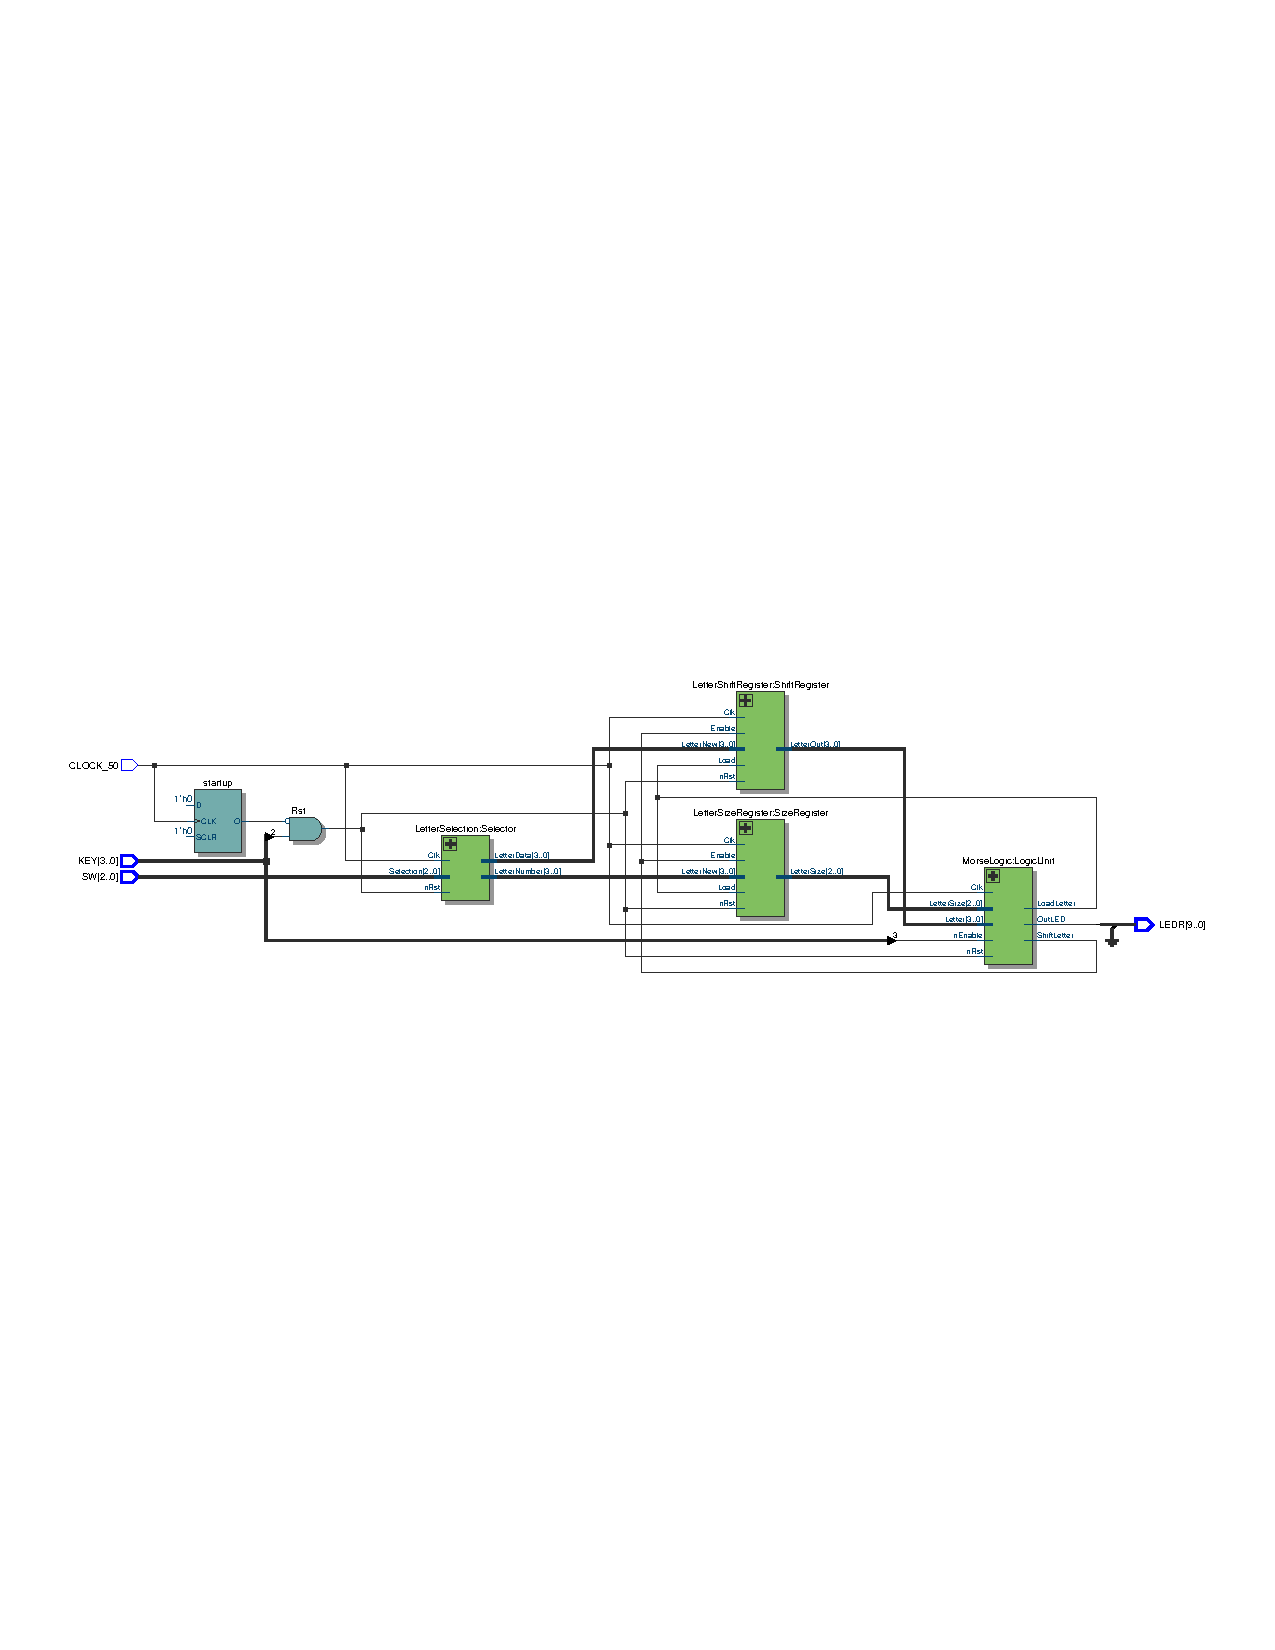
\includegraphics[width=1\textwidth]{Figures/Part3_RTL_TLE.jpg}
    \figcaption{RTL of the TLE}
    \label{fig:p3_RTL_TLE}
\end{figure}


\clearpage
\subsection{Results}
As read from figure~\ref{fig:p3_comp}, under "Logic utilization", this circuit uses a total of 28 logic elements to realize this configuration. That is not a lot as it is dealing with a 26 bit number and a 4 bit number, both with multiple comparators.

\begin{figure}[h]
    \centering
    \includegraphics[width=1\textwidth]{Figures/Part3_compiled.jpg}
    \figcaption{Compilation results from clock divider}
    \label{fig:p3_comp}
\end{figure}

A video of the counter counting would be the only true way to show how it functions. That can be found, also in the mentioned \linkgithub{GitHub} at {\small\verb|[PLK_lab/Lab04/Extra/Part3.mp4]|} if that is of interest. The pictures in figure~\ref{fig:p3_results} shows function but is limited.

\clearpage
\begin{figure}[h]
    \centering
    \begin{subfigure}[t]{0.45\textwidth}
        \centering
        \includegraphics[width=1\textwidth]{Figures/Part3_1.jpg}
        \caption{Disabled, reset low, value still}
        \label{fig:p3_1}
    \end{subfigure}
    \hfill
    \begin{subfigure}[t]{0.45\textwidth}
        \centering
        \includegraphics[width=1\textwidth]{Figures/Part3_2.jpg}
        \caption{Enabled, reset high, counting}
        \label{fig:p3_2}
    \end{subfigure}
    
    \begin{subfigure}[t]{0.45\textwidth}
        \centering
        \includegraphics[width=1\textwidth]{Figures/Part3_3.jpg}
        \caption{continuing to count}
        \label{fig:p3_3}
    \end{subfigure}
    \hfill
    \begin{subfigure}[t]{0.45\textwidth}
        \centering
        \includegraphics[width=1\textwidth]{Figures/Part3_4.jpg}
        \caption{Reset low, value set still at 0}
        \label{fig:p3_4}
    \end{subfigure}
    
    \figcaption{Testing results for clock divider}
    \label{fig:p3_results}
\end{figure}

\end{document}
